\documentclass{standalone}
\usepackage{tikz}

\begin{document}

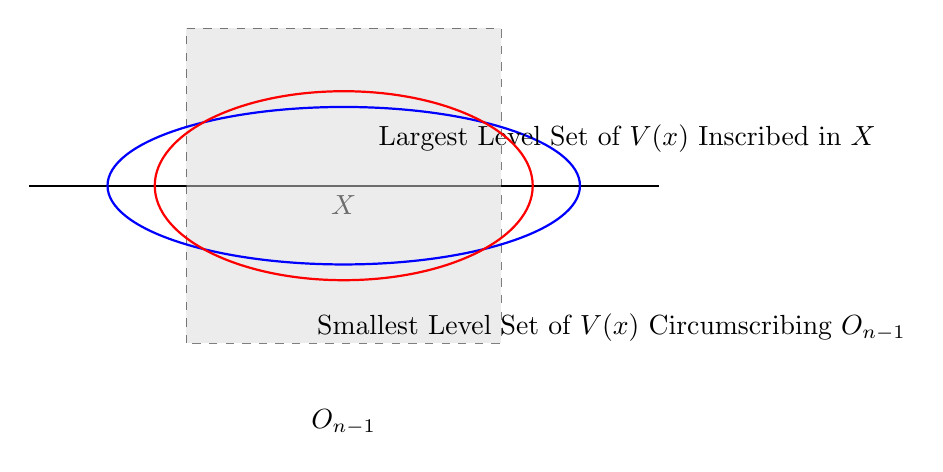
\begin{tikzpicture}[scale=2]
    % Define coordinates for the horizontal lines defining set X
    \coordinate (x1) at (-2, 0);
    \coordinate (x2) at (2, 0);

    % Draw the horizontal lines defining set X
    \draw[thick] (x1) -- (x2) node[midway, below] {$X$};

    % Define coordinates for the hatched box defining set O_{n-1}
    \coordinate (o1) at (-1, -1);
    \coordinate (o2) at (1, -1);
    \coordinate (o3) at (1, 1);
    \coordinate (o4) at (-1, 1);

    % Draw the hatched box defining set O_{n-1}
    \draw[dashed, fill=gray!30, opacity=0.5] (o1) rectangle (o3);
    \node at (0, -1.5) {$O_{n-1}$};

    % Draw the largest ellipse inscribed in X
    \draw[blue, thick, ->] (0, 0) ellipse (1.5 and 0.5);
    \node at (1.8, 0.3) {Largest Level Set of $V(x)$ Inscribed in $X$};

    % Draw the smallest ellipse circumscribing O_{n-1}
    \draw[red, thick, ->] (0, 0) ellipse (1.2 and 0.6);
    \node at (1.7, -0.9) {Smallest Level Set of $V(x)$ Circumscribing $O_{n-1}$};
\end{tikzpicture}

\end{document}